\documentclass{szzclass}

\usepackage{amsmath}
\usepackage{graphics}
\usepackage[export]{adjustbox}[2011/08/13]
\usepackage{subcaption}

% \usepackage[czech]{babel}
% \usepackage[margin=3cm]{geometry}
% \usepackage{wrapfig}

% spacing
\usepackage{titlesec}
% \titlespacing*{\section}{0pt}{1ex}{0.5ex}
\titlespacing*{\subsection}{0pt}{1ex}{0ex}
\usepackage{dependencies/szz-math}

\topic{Základy integrálního počtu (primitivní funkce, neurčitý integrál, Riemannův integrál (definice, vlastnosti a geometrický význam)).}
\author{Daniel Hampl}
\code{BI-SPOL-35}
\subject{ZMA}

\begin{document}
% \maketitle

\tableofcontents
\newpage

\section{Primtivní funkce}
Nechť $f$ je funkce definovaná na intervalu $(a,b)$, kde $-\infty\leq a < b\leq + \infty$. Funkci $F$ splňující podmínku
\begin{equation*}
F'(x) = f(x) \ \text{pro každé} \ x \in (a,b)\end{equation*}
nazýváme \textbf{primitivní funkcí} k funkci $f$ na intervalu $(a,b)$.


Nechť $F$ je primitivní funkcí k funkci $f$ na intervalu $(a,b)$.
Pak $G$ je primitivní funkcí k funkci $f$ na intervalu $(a,b)$
právě tehdy, když existuje konstanta $c \in \mathbb{R}$ taková, že
\begin{equation*}
G(x) = F(x) + c, \quad \text{pro každé} \ x\in(a,b).\end{equation*}

\section{Neurčitý integrál}

Nechť k funkci $f$ existuje primitivní funkce na intervalu $(a,b)$.
Množinu všech primitivních funkcí k funkci $f$ na $(a,b)$ nazýváme
neurčitým integrálem a značíme jej $\int f$ nebo $\int f(x) \,\mathrm{d}x$.


\subsection{Inverze}
\begin{equation*}
\int g'(x) \,\mathrm{d}x = g(x) + c, \quad x\in(a,b)\end{equation*}

\begin{equation*}
\left(\int f\right)'(x) = f(x), \quad x\in(a,b).\end{equation*}

\subsection{Operace}

\subsubsection{Sčtání a násobení konstantou}

\begin{equation*}
\int (f+g) = \int f + \int g \quad \text{a} \quad \int (\alpha f) = \alpha \int f,\end{equation*}

\subsubsection{Per partes}
Nechť funkce $f$ je diferencovatelná na intervalu $(a,b)$ a $G$ je primitivní funkce
k funkci $g$ na intervalu $(a,b)$ a konečně nechť existuje primitivní funkce k funkci
$f'G$. Potom existuje primitivní funkce k funkci $fg$ a platí
\begin{equation*}
\int fg = f G - \int f' G.\end{equation*}

\newpage

\subsubsection{Substituce}

\textbf{Věta o substituci I}\newline
Nechť pro funkce $f$ a $\varphi$ platí
\begin{itemize}
    \item $f$ má primitivní funkci $F$ na intervalu $(a,b)$,
    \item $\varphi$ je na intervalu $(\alpha,\beta)$ diferencovatelná,
    \item $\varphi\big((\alpha,\beta)\big) \subset (a,b)$
\end{itemize}
Pak funkce $f\big(\varphi(x)\big)\cdot\varphi'(x)$ má primitivní funkci na intervalu $(\alpha,\beta)$ a platí

\begin{equation*}
\int f\big(\varphi(x)\big)\cdot\varphi'(x) \,\mathrm{d}x = F\big( \varphi(x) \big).\end{equation*}


\textbf{Věta o substituci II}\newline
Nechť $f$ je definována na intervalu $(a,b)$ a nechť $\varphi$ je
bijekce\footnote{zobrazení $f$, které přiřazuje každému prvku $H_f$ právě jeden prvek z $D_f$}
intervalu $(\alpha,\beta)$ na $(a,b)$ s nenulovou konečnou derivací. Pak platí

\begin{equation*}
\int f(\varphi(t)) \varphi'(t) \,\mathrm{d}t = G(t) + C \quad \Longrightarrow \quad \int f(x) \,\mathrm{d}x = G\big(\varphi^{-1}(x)\big) + C\end{equation*}


\section{Riemannův integrál}
\subsection{Infimum}
Buď $A$ neprázdná zdola omezená podmnožina množiny reálných čísel.
Číslo $\alpha\in\mathbb{R}$ nazveme infimem množiny $A$, značíme
$\inf A$, právě když
\begin{enumerate}
    \item pro každé $x\in A$ platí $\alpha\leq x$ ($\alpha$ je dolní závora $A$),
    \item pokud $\beta\in \mathbb{R}$ také splňuje předchozí bod, pak $\beta\leq\alpha$ ($\alpha$ je největší dolní závora $A$).
\end{enumerate}

Pokud množina $A$ není zdola omezená, pak klademe $\inf A:=-\infty$. Pro prázdnou množinu klademe $\inf \emptyset:=+\infty$.


\subsection{Supremum}
Buď $A$ neprázdná zdola omezená podmnožina množiny reálných čísel.
Číslo $\alpha\in\mathbb{R}$ nazveme supremem množiny $A$, značíme
$\sup A$, právě když
\begin{enumerate}
    \item pro každé $x\in A$ platí $\alpha\geq x$ ($\alpha$ je horní závora $A$),
    \item pokud $\beta\in \mathbb{R}$ také splňuje předchozí bod,
    pak $\beta\geq\alpha$ ($\alpha$ je nejmenší honrní závora $A$).
\end{enumerate}

Pokud množina $A$ není shora omezená, pak klademe $\sup A:=+\infty$.
Pro prázdnou množinu klademe $\sup \emptyset:=-\infty$.

\newpage

\subsection{Norma dělení}
Buď dán interval $\langle a,b \rangle$. Konečnou množinu
$\sigma = \{x_0,x_1,\ldots,x_n\}$
takovou, že
$a = x_0 < x_1 < \cdots < x_n = b$
nazýváme dělením intervalu $\langle a,b \rangle$. Bodům $x_k, k=1,2,\ldots,n-1$
říkáme dělící body intervalu $\langle a,b \rangle$. Intervalu
$\langle x_{k−1},x_k \rangle$ říkáme částečný interval intervalu
$\langle a,b \rangle$ při dělení $\sigma$. Číslo

\begin{equation*}
\nu(\sigma) := \max \{ \Delta_k \mid k = 1,2,\ldots,n \}, \quad \text{kde} \quad \Delta_k := x_k - x_{k-1}, \ k = 1,2,\ldots,n,\end{equation*}

nazýváme \textbf{normou dělení} $\sigma$.

\subsection{Součet funkce}
Buďte funkce $f$ definovaná a omezená na intervalu $J=\langle a,b \rangle$ a $\sigma=\{x_0,x_1,…,x_n\}$ dělení intervalu $J$. Součty

\begin{equation*}
S(\sigma,f) := \sum_{i=1}^n \Delta_i \sup_{\langle x_{i-1},x_i\rangle} f \quad \text{a} \quad s(\sigma,f) := \sum_{i=1}^n \Delta_i \inf_{\langle x_{i-1},x_i\rangle} f\end{equation*}

nazýváme \textbf{horním součtem funkce} a \textbf{dolním součtem funkce} $f$ při dělení $\sigma$.

\begin{figure}[h]
    \begin{subfigure}{.5\textwidth}
        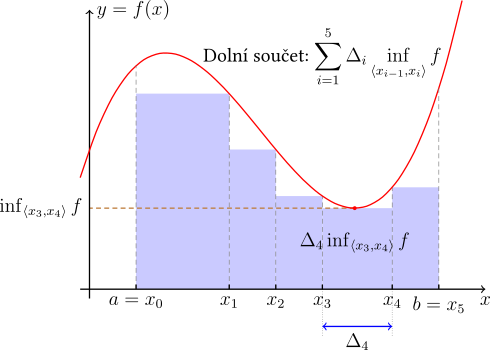
\includegraphics[width=\textwidth, center]{topics/bi-spol-35/images/fig_dolni_soucet.png}
    \end{subfigure}
    \begin{subfigure}{.5\textwidth}
        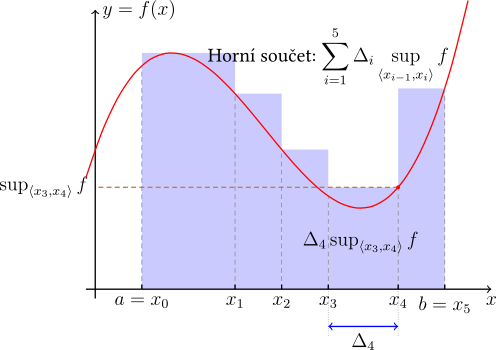
\includegraphics[width=\textwidth, center]{topics/bi-spol-35/images/fig_horni_soucet.png}
    \end{subfigure}
\end{figure}
% \begin{figure}[h]
%     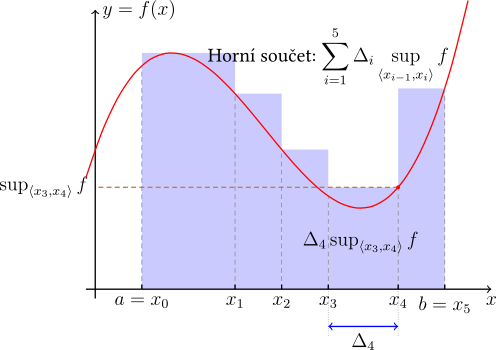
\includegraphics[width=.5\textwidth, center]{topics/bi-spol-35/images/fig_horni_soucet.png}
% \end{figure}

\subsection{Horní a dolní integrál}
Pro funkci $f$ definovanou a omezenou na uzavřeném intervalu $J=\langle a,b \rangle$ definujeme čísla

\begin{equation*}
\overline{\int_a^b} f(x) \,\mathrm{d}x := \inf\{ S(\sigma) \mid \sigma \ \text{dělení} \ J \} \ \text{a} \ \underline{\int_a^b} f(x) \,\mathrm{d}x := \sup\{ s(\sigma) \mid \sigma \ \text{dělení} \ J \}.\end{equation*}

a nazýváme \textbf{horním integrálem}, resp. \textbf{dolním integrálem}, funkce $f$ na intervalu $J$.

\newpage

\subsection{Definice Riemanova integrálu}

Pokud pro funkci $f$ definovanou a omezenou na uzavřeném intervalu $J$ platí

\begin{equation*}
\overline{\int_a^b} f(x)\,\mathrm{d}x = \underline{\int_a^b} f(x) \,\mathrm{d}x \in \mathbb{R},\end{equation*}

pak jejich společnou hodnotu nazýváme \textbf{Riemannovým integrálem}
funkce $f$ na intervalu $J$ a toto číslo značíme symboly

\begin{equation*}
\int_a^b f, \quad \text{případně} \quad \int_a^b f(x)\,\mathrm{d}x.\end{equation*}


Posloupnost dělení $\sigma_n$ nazveme \textbf{normální},
pokud pro její normy platí $\lim\limits_{n\to\infty} \nu(\sigma_n) = 0.$


\subsection{Postačujíící podmínka pro existenci RI}

Buď $f$ spojitá funkce na intervalu $\langle a,b \rangle$.
Potom existuje její Riemannův integrál na intervalu
$\langle a,b \rangle$. Pokud je navíc $(\sigma_n)$ normální
posloupnost dělení intervalu $\langle a,b \rangle$
potom limity

\begin{equation*}
\lim_{n\to\infty} s(\sigma_n, f) \quad \text{a} \quad \lim_{n\to\infty} S(\sigma_n,f)\end{equation*}

existují, a jsou rovny Riemannově integrálu funkce f na intervalu $\langle a,b \rangle$.


\subsection{Integrální součet}
Pro funkci f spojitou na uzavřeném intervalu $\langle a,b \rangle$
a dělení $\sigma={x_0,x_1,…,x_n}$, kde $x_0=a$ a $x_n=b$,
tohoto intervalu definujeme integrální součet funkce $f$
při dělení $σ$ předpisem

\begin{equation*}
\mathcal{J}(\sigma,f) = \sum_{i=1}^n f(\alpha_i) \Delta_i,\end{equation*}

kde $\alpha_i$ patří do intervalu $\langle x_{i−1},x_i\rangle$, $i=1,2,…,n$.

\subsubsection{Vztah s Riemannovým integrálem}

\begin{equation*}
\int_a^b f(x) \,\mathrm{d}x = \lim_{n\to\infty} \mathcal{J}(\sigma_n,f),\end{equation*}

\subsection{Vlastnosti}
\subsubsection{Aditivita integrálu}
Nechť $f$ a $g$ jsou spojité funkce na intervalu $\langle a,b \rangle$.
Potom pro Riemannův integrál funkce $f+g$ (která je také automaticky
spojitá na $\langle a,b \rangle$) platí

\begin{equation*}
\int_a^b (f+g)(x)\,\mathrm{d}x = \int_a^b f(x)\,\mathrm{d}x + \int_a^b g(x)\,\mathrm{d}x.\end{equation*}

\subsubsection{Multiplikativita integrálu}
Nechť f je spojitá na intervalu $\langle a,b \rangle$ a $c\in \mathbb{R}$
je konstanta. Potom pro Riemannův integrál funkce $cf$ platí

\begin{equation*}
\int_a^b (cf)(x)\,\mathrm{d}x = c \int_a^b f(x)\,\mathrm{d}x.\end{equation*}

\subsubsection{Aditivita integrálu v mezích}
Riemannův integrál funkce $f$ na intervalu $\langle a,b \rangle$
existuje, právě když pro každé $c\in\langle a,b \rangle$ existují
Riemannovy integrály funkce f na intervalech $\langle a,c \rangle$
a $\langle c,b \rangle$. V takovém případě navíc platí

\begin{equation*}
\int_a^b f(x)\,\d x  = \int_a^c f(x)\,\d x + \int_c^b f(x)\,\d x.\end{equation*}


\subsubsection{Nerovnosti mezi integrály}
Nechť jsou $f$ a $g$ spojité funkce na intervalu $\langle a,b \rangle$
a nechť platí nerovnost $f(x)\leq g(x)$ pro všechna
$x\in\langle a,b \rangle$. Potom pro jejich Riemannovy integrály platí

\begin{equation*}
\int_a^b f(x)\,\mathrm{d}x \leq \int_a^b g(x)\,\mathrm{d}x.\end{equation*}


\subsubsection{Newtonova formule}
Nechť f je funkce spojitá na intervalu $\langle a,b \rangle$ s primitivní funkcí F. Pak platí rovnost
\begin{equation*}
\int_a^b f(x) \,\mathrm{d}x = F(b) - F(a) =: \Big[ F(x) \Big]_a^b.\end{equation*}


\subsection{Zobecněný RI}
Nechť f je funkce definovaná na intervalu $\langle a,b )$
pro nějaké $a\in\mathbb{R}$ a $b\in(a,+\infty\rangle$,
která je Riemanovsky integrabilní na intervalu$\langle a,c \rangle$
pro každé $c\in(a,b)$. Pokud existuje konečná limita

\begin{equation*}
\lim_{c \to b_-} \int_a^c f(x)\, \d x,\end{equation*}

pak její hodnotu značíme

\begin{equation*}
\int_a^b f(x)\, \d x,\end{equation*}

nazýváme zobecněným Riemannovým integrálem funkce $f$
na intervalu $\langle a,b )$ a říkáme, že integrál
$\int_a^b f(x)\, \d x$ konverguje.

\subsection{Vlastnosti RI}
Nechť $f$ je funkce spojitá na uvažovaných intervalech.
\begin{itemize}
    \item Je-li $f$ sudá funkce na $\langle -a,a \rangle$, pak
    $\displaystyle\int_{-a}^a f(x) \mathrm{d}x = 2 \int_0^a f(x) \mathrm{d}x$
    \item Je-li $f$ lichá funkce na $\langle -a,a \rangle$, pak
    $\displaystyle\int_{-a}^a f(x) \mathrm{d}x = 0$
    \item Je-li $f$ periodická na $\mathbb{R}$ s periodou $T$, pak pro každé $a,b\in\mathbb{R}$ platí
    $\displaystyle\int_a^{a+T} f(x)\mathrm{d}x = \int_b^{b+T} f(x) \mathrm{d}x$
\end{itemize}

\subsection{Výpočet obsahů plošných útvarů}
Nechť $f$ a $g$ jsou funkce spojité na $\langle a,b \rangle$
takové, že $f(x)\geq g(x)$ pro každé $x\in\langle a,b \rangle$.
Pak obsah plochy $P$ ohraničené přímkami $x=a$ a $x=b$ a grafy
funkcí $f$ a $g$ je roven

\begin{equation*}
P = \int_a^b \big( f(x) - g(x) \big) \,\mathrm{d}x.\end{equation*}

\begin{figure}[h]
    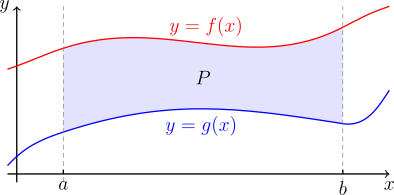
\includegraphics[width=.5\textwidth, center]{topics/bi-spol-35/images/fig_vypocet_plochy.png}
\end{figure}



\newpage
\section{Tabulky}

\begin{figure}[h]
    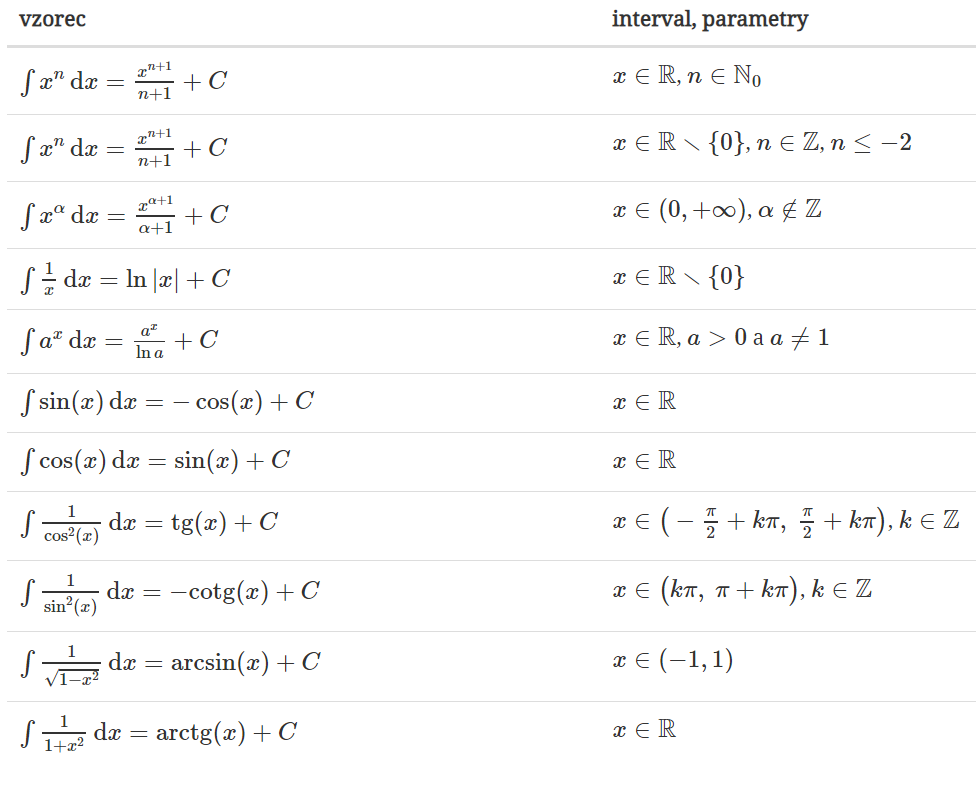
\includegraphics[width=\textwidth, center]{topics/bi-spol-35/images/integraly.png}
\end{figure}

\end{document}